\section{RAILS analyse} \label{app:railsAnalysis}

\begin{figure}[ht]
    \centering
    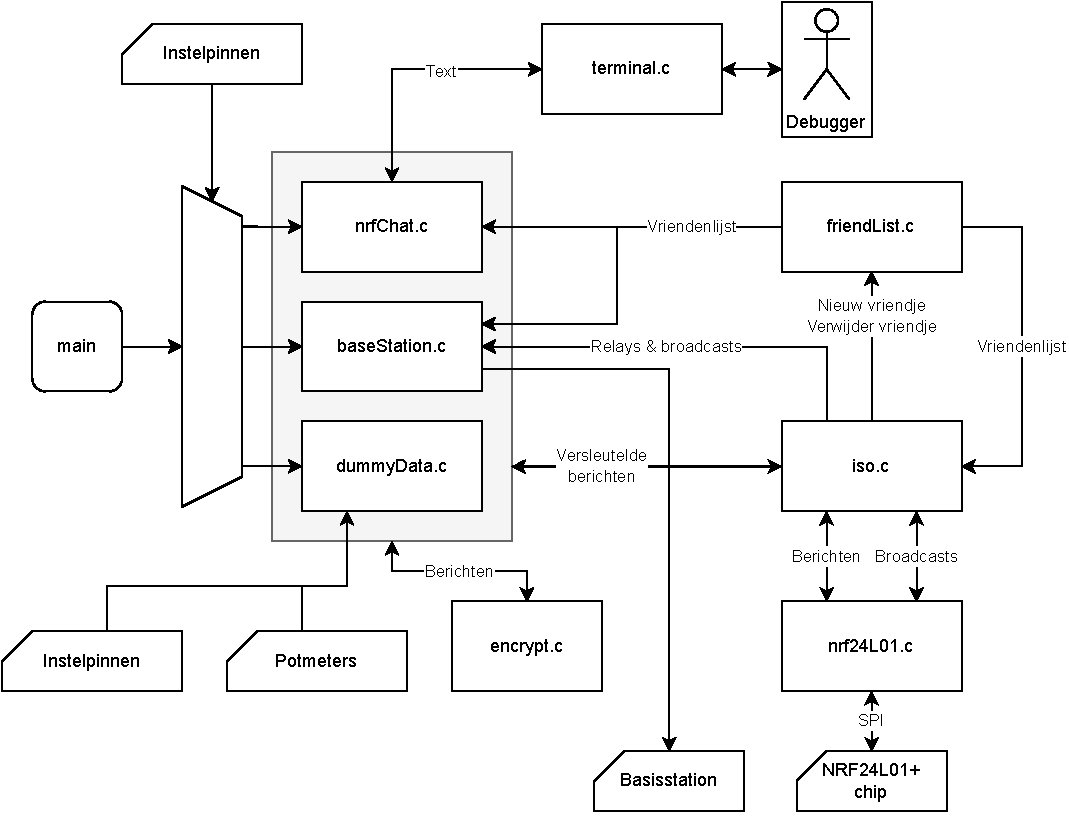
\includegraphics[width=\textwidth]{img/xmegablokshema}
    \caption{Een blokschema van de XMega.}
    \label{fig:xmegaBlokSchema}
\end{figure}

\noindent
In deze analyse zal er worden gekeken naar welke aspecten van de soft/hardware er in de volgende ontwikkel cyclus verbeterd kunnen worden. De analyse methode die wordt gebruikt is de RAILS analyse. Een RAILS analyse bestaat uit de volgende onderdelen:
\begin{itemize}
    \item Revisie
    \item Algoritmes
    \item Interactie
    \item Lookup tabellen
    \item Slaap
\end{itemize}
De bovengenoemde onderdelen zullen in de rest van deze appendix worden beschreven.

\subsection{Revisie}

Voor de revisie is het volledige systeem van de XMega in een blokschema verwerkt. Deze is te zien in \autoref{fig:xmegaBlokSchema}. Het blokschema bevat alle functionele blokken van de code. Deze zijn vanaf het begin van het project al onderverdeeld in aparte C bestanden, waardoor de code erg overzichtelijk is.


\subsection{Algoritmes}

Er is uitgebreid nagedacht over de algoritmes in de code. De belangrijkste algoritmes die het meeste tijd innemen bevinden zich in het iso gedeelte en de vriendenlijst. De vriendenlijst gebruikt een array met zogenaamde `gaten' er in, die ervoor zorgen dat de lijst niet elke keer opgeschoven hoeft te worden wanneer er een vriendje verwijdert wordt. Hier is meer over te lezen in \autoref{sec:vriendjes}.

Een snapshot wordt elke keer dat deze verstuurd wordt opnieuw opgebouwd. Dit is omdat de snapshot maar één keer per seconde gestuurd wordt. Aangezien het netwerk vaak meer dan één node bevat, zullen snapshots een stuk vaker ontvangen dan verzonden worden. Hierdoor zou het continu bijhouden van de snapshot die verstuurd moet worden, terwijl ook de vriendenlijst bijgehouden wordt, qua snelheid nadelig zijn.

Wanneer er een vriendje toe wordt gevoegd aan de lijst start het algoritme altijd met zoeken bij het begin van de array. Hier is ruimte voor een kleine optimalisatie. Als continu de laagste lege index bijgehouden wordt, (deze zou bijgewerkt worden wanneer er een vriendje verwijdert wordt) hoeft het algoritme niet elke keer door de volledige array. Dit zou niet veel schelen, maar het is toch net iets efficiënter.


\subsection{Interactie}
Dit hoofdstuk beschrijft de wisselwerking tussen de hardware, software en digitale onderdelen. Het proof of concept bestaat op het moment voornamelijk uit software. De enige hardware vereisten die er op dit moment zijn, zijn:
\begin{itemize}
    \item XMega microcontroller.
    \item SPI verbinding tussen de XMega en de NRF24L01+.
    \item UART naar USB omzetting.
    \item ADC voor de potentiometer.
\end{itemize}
De verdeling tussen de hardware en de software is redelijk logisch op het moment. Het is namelijk vrij lastig om gewild draadloze communicatie op te zetten die enkel door software wordt geïmplementeerd. Afhankelijk van de resultaten van dit proof of concept kan het logisch worden om de communicatie stack te implementeren in een ASIC. Voordat dit gedaan wordt moet het proof of concept eerst verder zijn uitgewerkt.

De software bestaat uit verschillende abstractie lagen. Het is wel aan te raden om een hardware abstractielaag te schrijven. Dit om ervoor te zorgen dat het makkelijk is om van microcontroller te kunnen wisselen.

Op dit moment is er geen speciale hardware ontwikkeld voor de implementatie van het proof of concept. Het is aan te raden om dit in de toekomst wel te doen. Met name is het aan te raden om hardware te ontwikkelen voor de sensor nodes en de basisstation nodes. Bij het ontwikkelen van de hardware voor de sensor nodes is het aan te raden om er voor te zorgen dat het makkelijk is om nep data te gebruiken, dan wel echte sensoren aan te sluiten. Deze aanbeveling wordt gedaan om er voor te zorgen dat de hardware niet te vaak aangepast hoeft te worden in de ontwikkeling van het proof of concept.

\subsection{Lookup tabellen}
Aangezien de vriendjes worden opgeslagen in een array die groot genoeg is om het maximum aantal vriendjes op te kunnen slaan, zou het voor de hand liggen om hier ook een lookup tabel voor te gebruiken. De vriendjes kunnen dan op de index van hun ID opgeslagen worden.
\begin{table}[ht]
    \centering
    \begin{tabular}{c|cc}
    Operatie                    & Snelheid nu & Snelheid met lookup tabel \\
    \hline \hline
    Vriendje toevoegen          & \makecell{$O(s)$ \\ $\Theta(n)$ \\ $\Omega(1)$} & \makecell{$O(1)$ \\ $\Theta(1)$ \\ $\Omega(1)$} \\
    \hline
    Vriendje verwijderen        & \makecell{$O(1)$ \\ $\Theta(1)$ \\ $\Omega(1)$} & \makecell{$O(1)$ \\ $\Theta(1)$ \\ $\Omega(1)$} \\
    \hline
    Vriendje vinden in lijst    & \makecell{$O(s)$ \\ $\Theta(n)$ \\ $\Omega(1)$} & \makecell{$O(1)$ \\ $\Theta(1)$ \\ $\Omega(1)$} \\
    \hline
    Door hele lijst heen gaan   & \makecell{$O(s)$ \\ $\Theta(n)$ \\ $\Omega(n)$} & \makecell{$O(s)$ \\ $\Theta(s)$ \\ $\Omega(n)$} \\
    \hline
    \end{tabular}
    \caption{De big O, big $\Theta$ en big $\Omega$ snelheid van de operaties die over de vriendjeslijst worden uitgevoerd. `n' is hier het aantal bekende vriendjes, `s' is de grootte van de array.}
    \label{tab:speedOfTheFriends}
\end{table}

De asymptotische snelheid van de operaties is genoteerd in \autoref{tab:speedOfTheFriends}. Hier is te zien dat, wanneer vriendjes worden opgeslagen op de index van hun ID, het algoritme bijna altijd sneller is. De enige situatie waarin dit trager is, is wanneer er door de volledige array heen wordt gezocht. Deze operatie gebeurt een enkele keer wanneer er een snapshot ontvangen wordt, een enkele keer wanneer er een snapshot opgebouwd wordt en elke keer wanneer er een vriendje gedeactiveerd wordt. De andere operaties gebeuren veel vaker. Het is dus aan te raden om te testen of deze methode van vriendjes opslaan daadwerkelijk sneller is.

\subsection{Slaap}
In dit proof of concept worden sensor nodes gebruikt. Het is de verwachting dat deze sensor nodes in de toekomst via een batterij gevoed gaan worden. Om ervoor te zorgen dat de levensduur van de batterij gevoede nodes langer is, zal er gekeken worden hoe er in de toekomst energie bespaard kan worden. Omdat op dit moment alleen nog software is ontwikkeld zal de energie besparingsoptimalisatie op de software zijn gericht. 

Op de XMega zijn er drie manieren om energie te besparen\footnote{De voedingsspanning wordt buiten beschouwing gelaten omdat dit proof of concept gebruik maakt van het XMega ontwikkelbord van de HvA.}:
\begin{itemize}
    \item De kloksnelheid verlagen.
    \item De XMega in een slaapstand te zetten.\footnote{De energiebesparing hangt af van welke slaapstand er wordt gebruikt \cite{XMegaDatasheet}.}
    \item Ongebruikte peripherals van de XMega uitzetten.
\end{itemize} 
Het is belangrijk om op te merken dat als de kloksnelheid wordt verlaagd dit niet altijd tot een energie besparing leidt. Deze onzekerheid vindt plaats op het moment dat de XMega gebruik maakt van slaapstanden. 

Op dit moment wordt er geen gebruik gemaakt van de slaapstanden en is de kloksnelheid van de XMega 32MHz. Wanneer de slaapstanden worden gebruikt, verbruikt de XMega een minimale hoeveelheid energie \cite{XMegaDatasheet}. Hierdoor is het aan te raden om in een volgende software revisie van de sensor nodes gebruik te gaan maken van de slaapstanden van de XMega. 
% \fbox{
%     \centering
%     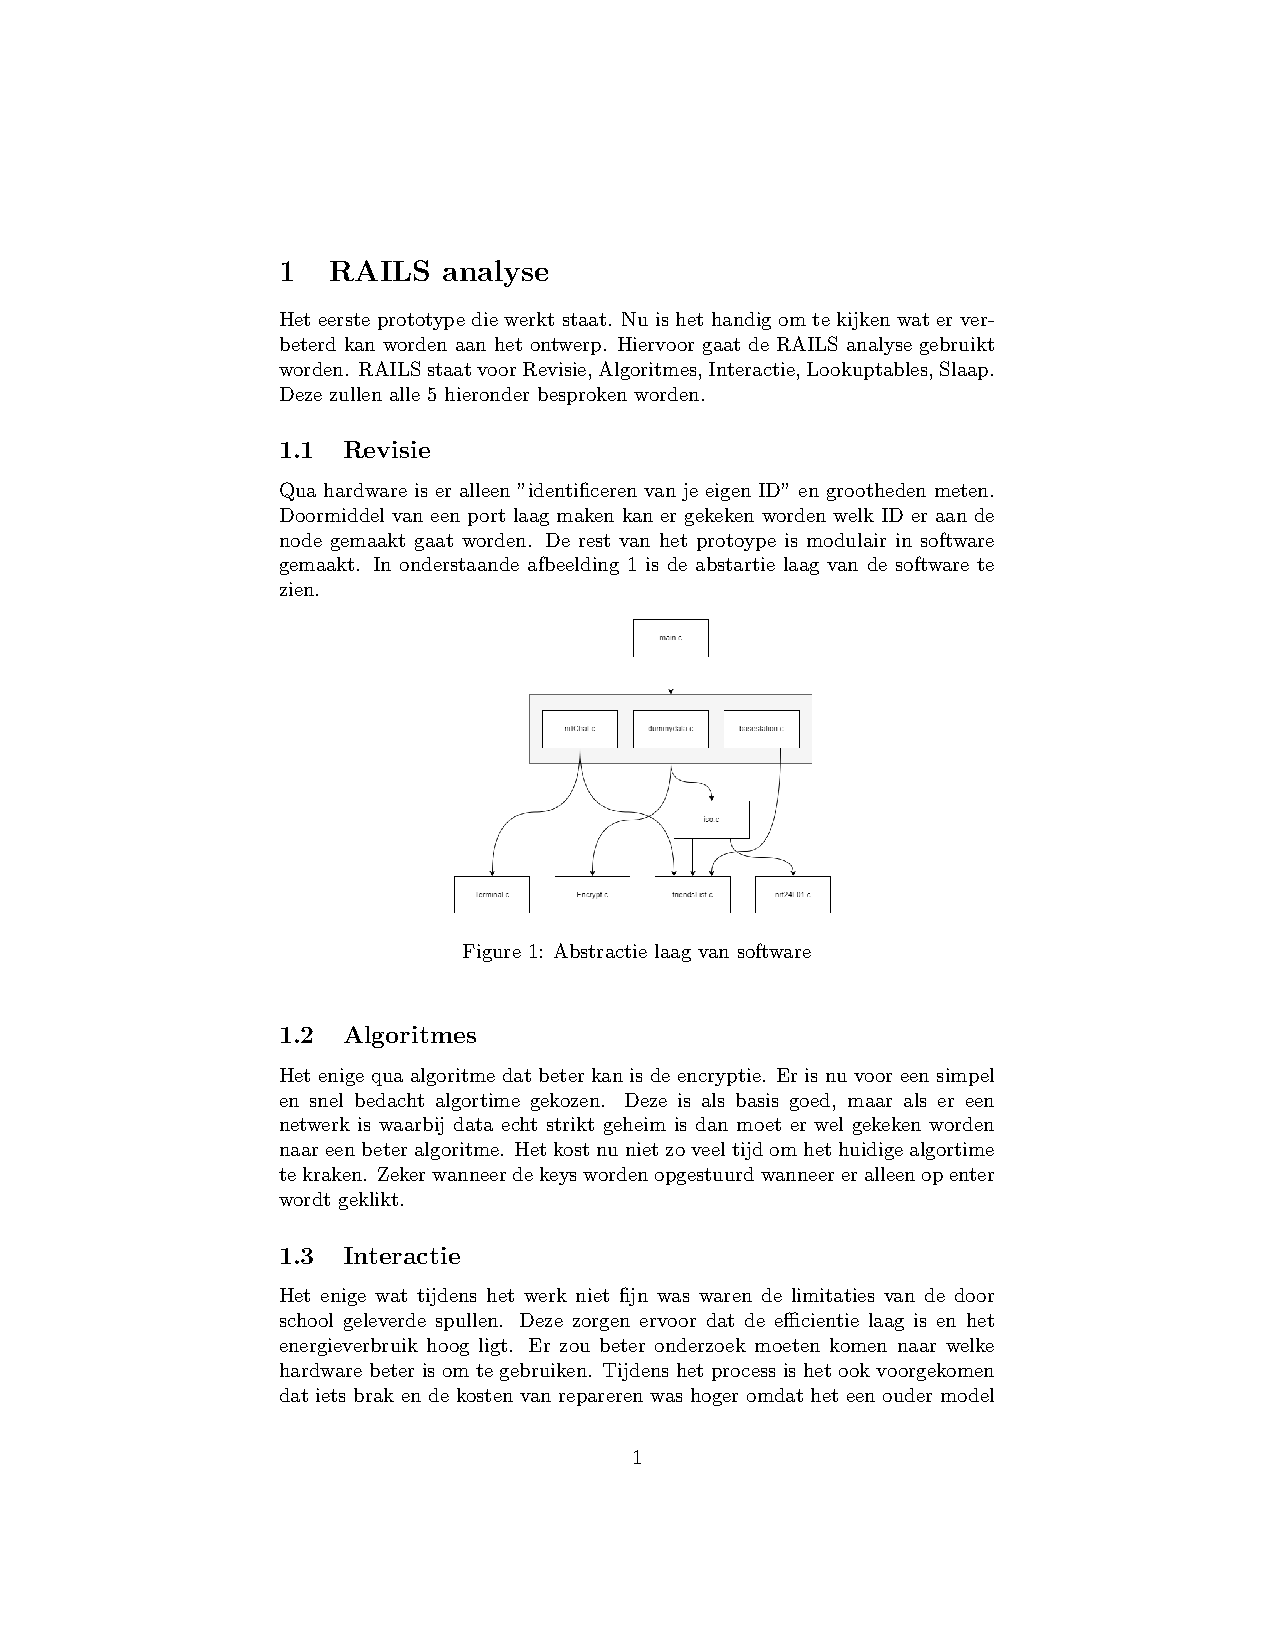
\includegraphics[page=1,scale=0.7]{img/RAILS.pdf}
% }

% \fbox{
%     \centering
%     \includegraphics[page=2,scale=0.7]{img/RAILS.pdf}
% }